\documentclass{article}

\usepackage{graphicx}
\usepackage{tikz}
\usepackage{tikzsymbols}
\usetikzlibrary{calc,patterns,shapes.geometric}
\pagestyle{empty}
\usepackage[margin=0pt]{geometry}
\geometry{papersize={14in,12in}}

\def\centerarc[#1](#2)(#3:#4:#5){\draw[#1] ($(#2)+({#5*cos(#3)},{#5*sin(#3)})$) arc (#3:#4:#5);}

\begin{document}
	\begin{figure}
		\centering
		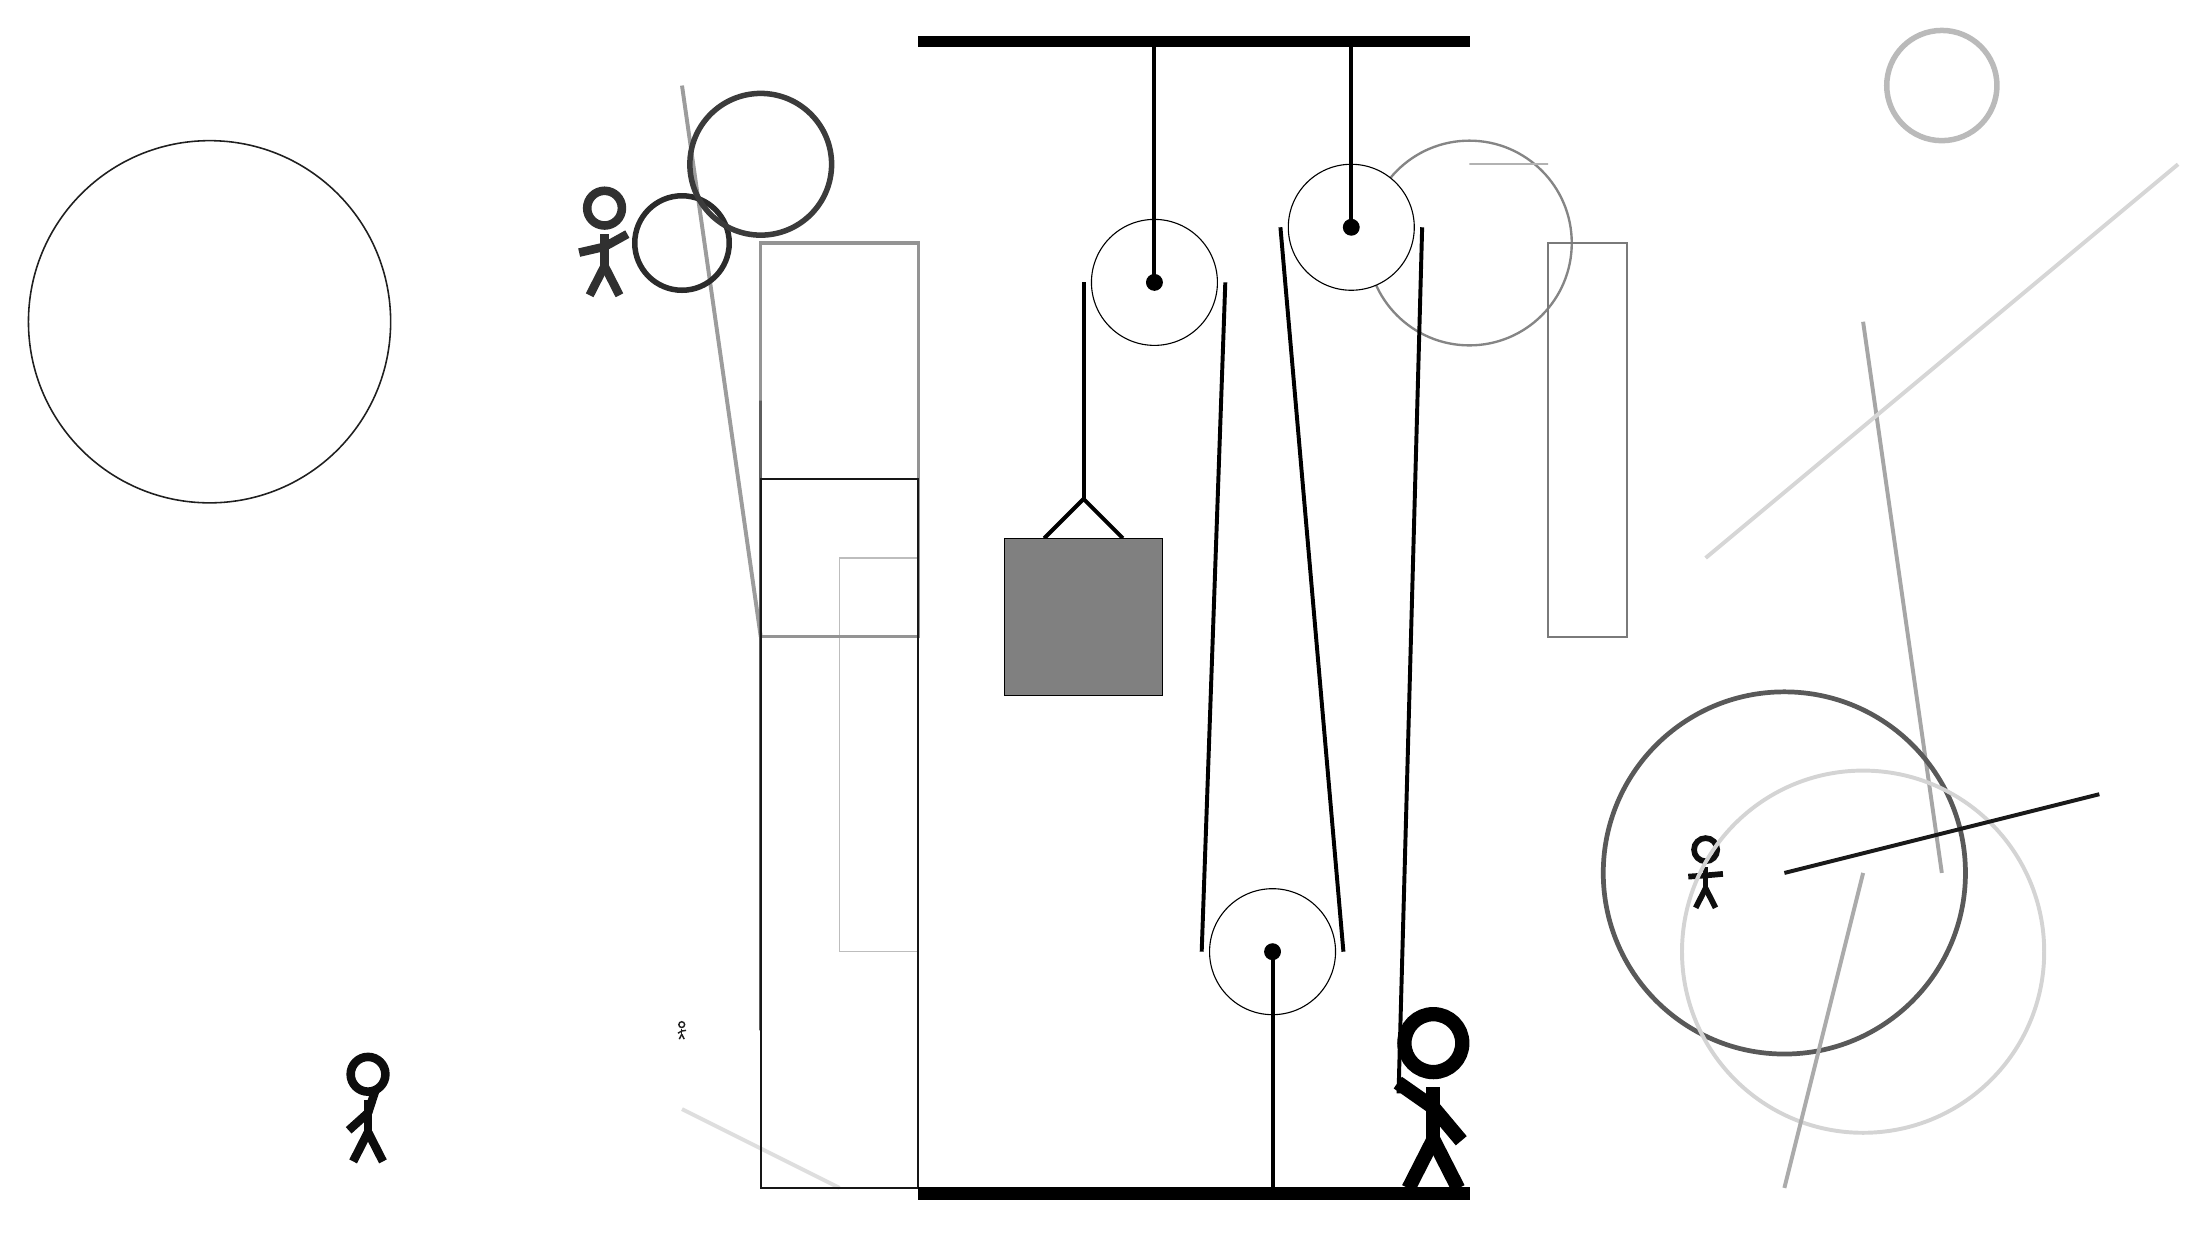
\begin{tikzpicture}
			%%%%% START %%%%%
			
			\draw[fill=black] (-2, 11.5) rectangle (5, 11.625);
			
			\draw [line width=0.3mm, color=black!48](5, 9) circle (1.3);
			
			\draw[line width=0.5mm, color=black!39](-4, 4) -- (-5, 11);
			\draw[line width=0.2mm, color=black!26] (-3, 0) rectangle (-2, 5);
			\node[line width=0.3mm, color=black!94] at (8, 1) {\Strichmaxerl[4][4][5]};
			\node[line width=0.7mm, color=black!81] at (-6, 9) {\Strichmaxerl[6][13][29]};
			\draw[line width=0.4mm, color=black!42] (-4, 9) rectangle (-2, 4);
			\draw[line width=0.5mm, color=black!35](10, 8) -- (11, 1);
			\draw[line width=0.5mm, color=black!13](-5, -2) -- (-3, -3);
			\draw [line width=0.6mm, color=black!65](9, 1) circle (2.3);
			
			\draw [line width=0.7mm, color=black!83](-5, 9) circle (0.6);
			
			\node[line width=0.2mm, color=black!95] at (-9, -2) {\Strichmaxerl[6][42][72]};
			
			\draw[line width=0.4mm, color=black!63] (-4, 7) rectangle (-4, -1);
			\draw [line width=0.2mm, color=black!88](-11, 8) circle (2.3);
			
			\draw [line width=0.7mm, color=black!27](11, 11) circle (0.7);
			\draw[line width=0.5mm, color=black!16](8, 5) -- (14, 10);
			\draw [line width=0.5mm, color=black!17](10, 0) circle (2.3);
			\draw [line width=0.7mm, color=black!77](-4, 10) circle (0.9);
			\draw[line width=0.2mm, color=black!52] (7, 9) rectangle (6, 4);
			\draw[line width=0.3mm, color=black!91] (-4, -3) rectangle (-2, 6);
			\draw[line width=0.3mm, color=black!30] (5, 10) rectangle (6, 10);
			\draw[line width=0.5mm, color=black!90](9, 1) -- (13, 2);
			
			\node[line width=0.4mm, color=black!88] at (-5, -1) {\Strichmaxerl[1][30][9]};
			
			\draw[line width=0.5mm, color=black!33](9, -3) -- (10, 1);
			
			\draw (1, 8.5) circle (0.8);
			\draw[fill=black] (1, 8.5) circle (0.1);
			\draw[line width=0.5mm]  (1, 11.5) -- (1, 8.5);
			
			\draw[fill=white](2.5, 0.0) circle (0.8);
			\draw[fill=black] (2.5, 0.0) circle (0.1);
			\draw[line width=0.5mm]  (2.5, -3) -- (2.5, 0.0);
			
			\draw[fill=white](3.5, 9.2) circle (0.8);
			\draw[fill=black] (3.5, 9.2) circle (0.1);
			\draw[line width=0.5mm] (3.5, 11.5) -- (3.5, 9.2);
			
			\draw[line width=0.5mm] (-0.4, 5.25) -- (0.1, 5.75) -- (0.6, 5.25);
			\draw[fill=black!50] (-0.9, 5.25) rectangle (1.1, 3.25);
			
			\draw[line width=0.5mm] (0.1, 8.5) -- (0.1, 5.75);
			\centerarc[line width=0.5mm](1, 8.5)(0:180:0.9);
			\draw[line width=0.5mm](1.9, 8.5) -- (1.6, 0.0);
			\centerarc[line width=0.5mm](2.5, 0.0)(180:360:0.9);
			\draw[line width=0.5mm](3.4, 0.0) -- (2.6, 9.2);
			\centerarc[line width=0.5mm](3.5, 9.2)(0:180:0.9);
			\draw[line width=0.5mm](4.4, 9.2) -- (4.1, -1.8);
			
			\node at (4.5, -1.9) {\Strichmaxerl[10][-35][-50]};
			
			\draw[fill=black] (-2, -3) rectangle (5, -3.15);
			
			%%%%% END %%%%%
		\end{tikzpicture}
	\end{figure}	
\end{document}